\begin{block}{Intro to Data Consistent Inversion}
\centering
        \heading{Solving Stochastic Inverse Problems} 
            %{\large How do we update initial descriptions of uncertainty using model predictions and data?}

        %\heading{Background}
             %{\large \emph{Data Consistent Inversion} is a Measure-Theoretic Framework for the solution of stochastic inverse problems. }
             {\large \textbf{Data-Consistent Inversion} is a novel framework that uses push-forward and pull-back measures to ensure solutions are consistent with the observed distribution of data.}

        %\heading{Question} 
         %    {\large \emph{How do we cast a \textbf{Parameter Identification} problem in the context of Data-Consistent Inversion?} }
\vspace{0.5cm}
\heading{The Approach}
\[ \scalebox{1.5}{$\dci$} \]


\end{block}


\begin{block}{Which Stochastic Inverse Problem?}
\centering

% \vspace{1cm}
% \heading{Quantity of Interest Map}
%     \emph{\large A Functional Relating \textbf{Predictions} and \textbf{Data}}
%     \large
%     \begin{itemize}
%        \itembox{Ideal} $Q \left (\param, \noise \right ) = F \left ( \obs(\param), \data(\noise) \right )$
%        \itembox{Theoretical} $Q \left ( \pspace, \nspace \right ) =: \dspace_\mathcal{T} \subset \RR$
%        \itembox{Practical} $Q \left (\param \right ) = F \left ( \obs(\param), \data^\dagger \right )$
%        \itembox{Computable} $Q \left ( \pspace \right ) =: \dspace_\mathcal{C} \subset \dspace_\mathcal{T}$
%     \end{itemize}
    \begin{figure}
        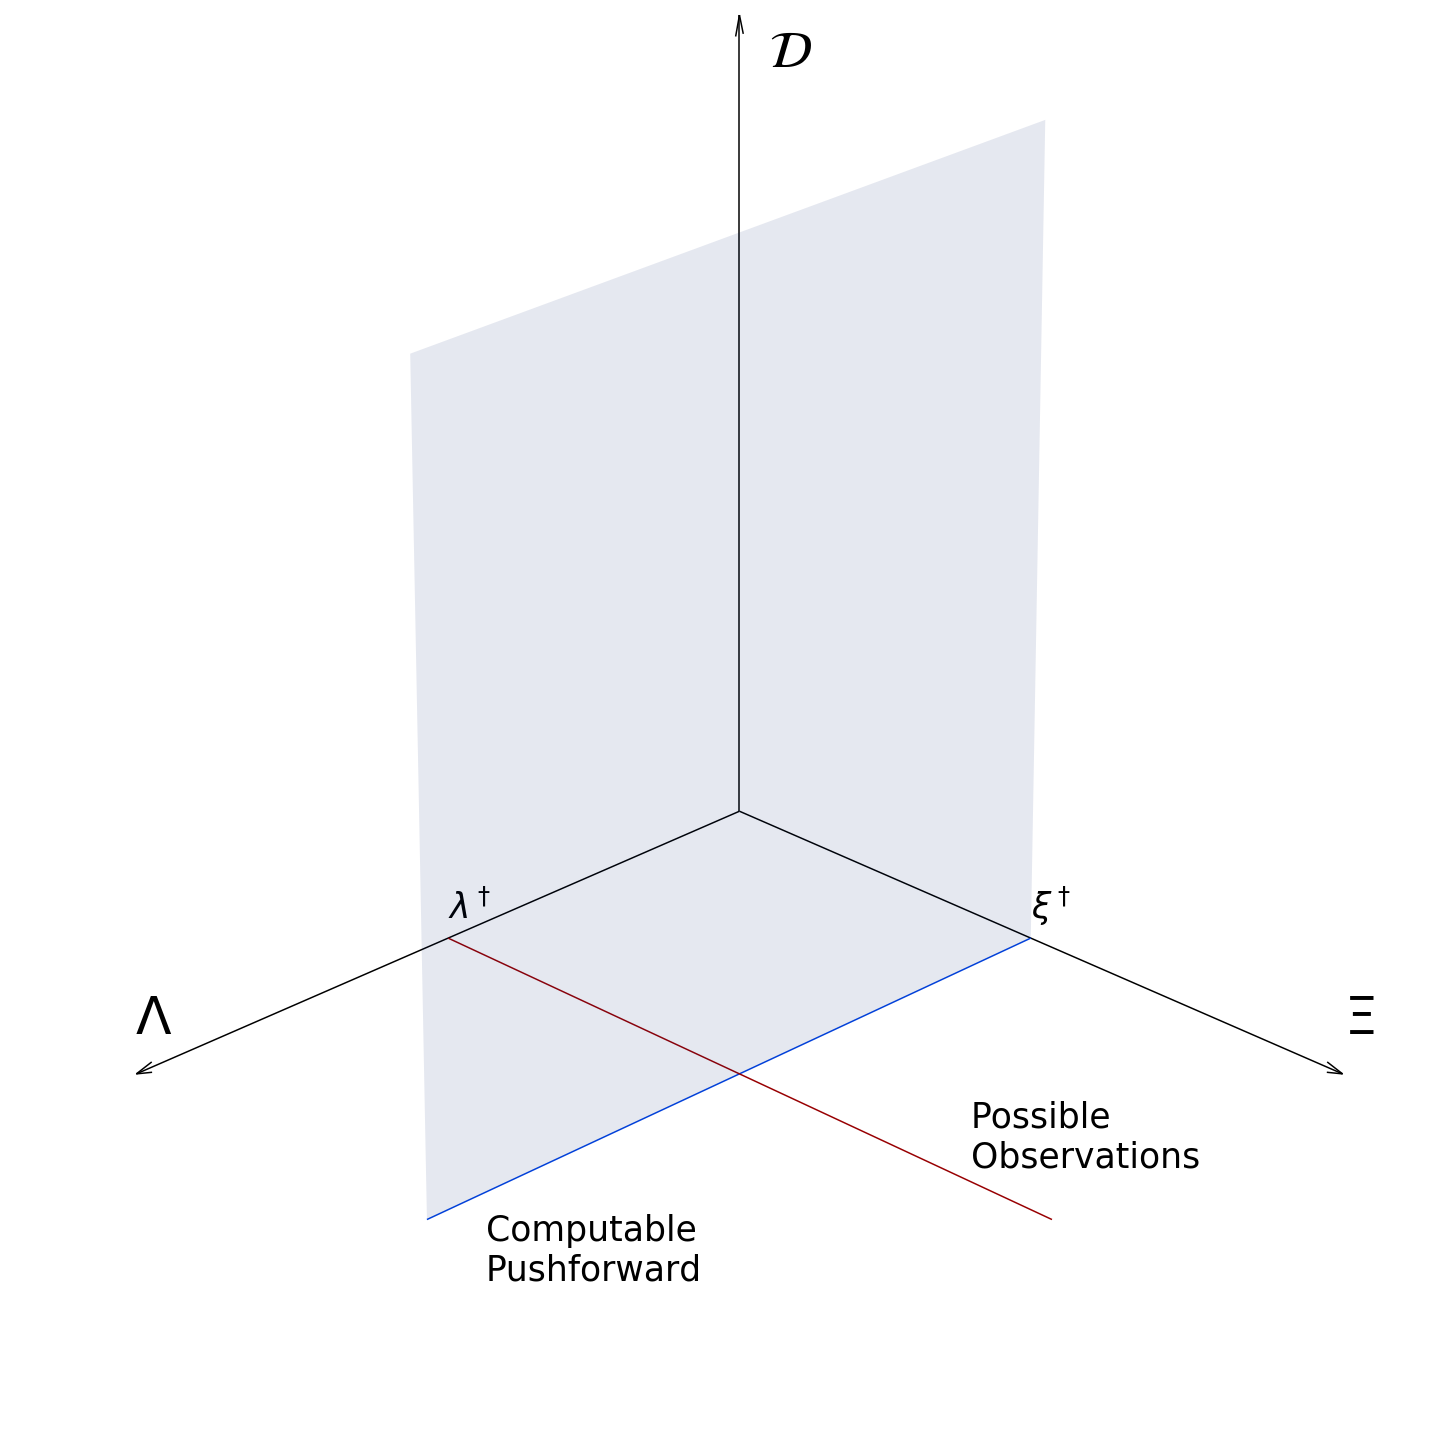
\includegraphics[height=23cm]{figures/diagram}
    \caption{\large \emph Do you want to solve for a single parameter value or for a parameter distribution?}
    \end{figure}


% \vspace{1cm}
% \heading{Observed Distribution}
% {\large \emph Given a functional, what measure do we invert?}

% \Large
%     $Q(\param^\dagger, \noise) \sim \observed$ when we allow $\noise$ to vary over $\nspace$
%     \begin{table}
%       \centering
%       {\setlength{\tabcolsep}{0.25em}
%       \begin{tabular}{c <{\hspace{1pc}} c >{\hspace{1pc}} c}
%         %\toprule
%         %\large
%         \textbf{$F(\obs(\param), \data^\dagger)$} & \textbf{$\noise$} & {$\observed$} \\
%         \midrule
%         $\frac{1}{\sigma\sqrt{D}} \large\sum \left( \obs_i\lam - \data_i^\dagger \right)$ & $ \noise \sim L^2$ & $N(0,1) $ \\[1.5ex]
%         $\frac{1}{\sigma^2} \large\sum \left ( \obs_i\lam - \data_i^\dagger \right)^2$ & $ \noise \sim N(0,\sigma^2) $ & $\chi^2 (D)$ \\[1.5ex]
%         $\frac{1}{\sigma^2 D} \large\sum \left ( \obs_i\lam - \data_i^\dagger \right)^2$ & $ \noise \sim N(0,\sigma^2) $ & $ \Gamma \left ( D/2, D/2) \right ) $ \\
%         \normalsize\vdots & \normalsize\vdots & \normalsize\vdots \\
%         %\bottomrule
%       \end{tabular}
%       }
%       \caption{Choices of $F$ and associated $\observed$ for stochastic inverse problem with $\data^\dagger = \obs_i(\param^\dagger) + \xi_i^\dagger$
% }
%     \end{table}

%
\end{block}
